\documentclass[11pt,a4paper]{article}

\usepackage[T1]{fontenc}
\usepackage[utf8]{inputenc}
\usepackage{lmodern}
\usepackage[final]{microtype}
\usepackage[a4paper,margin=1in]{geometry}
\usepackage{amsmath,amssymb}
\usepackage{graphicx}
\usepackage{booktabs}
\usepackage{setspace}
\usepackage[font=small,labelfont=bf,labelsep=period,skip=6pt]{caption}
\usepackage[round,authoryear]{natbib}
\usepackage{titlesec}
\usepackage{enumitem}
\usepackage{xcolor}
\usepackage{xurl}
\usepackage[colorlinks=true,linkcolor=linkblue,citecolor=linkblue,urlcolor=linkblue]{hyperref}

\definecolor{linkblue}{HTML}{1F4E8C}
\hypersetup{pdftitle={A Four-Asset Efficient Frontier in Three Dimensions: Estimation Error and an Out-of-Sample Test},pdfauthor={Mael Tok}}
\setstretch{1.12}
\titleformat{\section}{\normalfont\large\bfseries}{\thesection}{0.8em}{}
\titlespacing*{\section}{0pt}{1.3\baselineskip}{0.45\baselineskip}
\setlist{itemsep=2pt,topsep=4pt}
\bibpunct{(}{)}{;}{a}{}{,}
\frenchspacing
\newcommand{\tabnote}[1]{\par\vspace{5pt}\begin{minipage}{\linewidth}\setstretch{1.0}\footnotesize\textit{Notes:} #1\end{minipage}}

% generated by code/tables.py -- do not edit
\newcommand{\nWeeks}{522}
\newcommand{\rfMean}{2.0}
\newcommand{\nDailyObs}{2{,}444}
\newcommand{\goldCorrGood}{0.97}
\newcommand{\goldCorrBad}{0.92}
\newcommand{\aruMeanTotal}{39}
\newcommand{\aruCagr}{15}
\newcommand{\aruVol}{74}
\newcommand{\nvdaCagr}{80}
\newcommand{\msNvda}{40}
\newcommand{\msSgln}{54}
\newcommand{\msAru}{5}
\newcommand{\msSharpe}{1.60}
\newcommand{\msVol}{22}
\newcommand{\vOneSharpe}{1.56}
\newcommand{\vOneVol}{18}
\newcommand{\ewSharpe}{1.21}
\newcommand{\gridN}{12{,}341}
\newcommand{\gridShareTen}{19}
\newcommand{\gridShareFive}{5.5}
\newcommand{\nearNvdaLo}{25}
\newcommand{\nearNvdaHi}{75}
\newcommand{\nearSglnLo}{15}
\newcommand{\nearSglnHi}{72.5}
\newcommand{\nearVooHi}{20}
\newcommand{\ratioVoo}{1.22}
\newcommand{\ratioAru}{0.86}
\newcommand{\ratioNvda}{0.98}
\newcommand{\ratioSgln}{1.01}
\newcommand{\ratioMin}{0.86}
\newcommand{\ratioMax}{1.23}
\newcommand{\ratioShareAbove}{65}
\newcommand{\skewAru}{1.30}
\newcommand{\skewVoo}{-0.64}
\newcommand{\cvarGain}{1.7}
\newcommand{\cvarVolCost}{1.3}
\newcommand{\cvarMaxGap}{14}
\newcommand{\rollWeeks}{434}
\newcommand{\rollRebal}{109}
\newcommand{\rollExpected}{1.53}
\newcommand{\rollMs}{0.88}
\newcommand{\rollEw}{0.92}
\newcommand{\rollRp}{1.10}
\newcommand{\rollMv}{0.92}
\newcommand{\rollMsDd}{47}
\newcommand{\rollRpDd}{26}
\newcommand{\rollMsTurn}{93}
\newcommand{\rollRpTurn}{33}
\newcommand{\rollMsLo}{0.30}
\newcommand{\rollMsHi}{1.50}
\newcommand{\diffEst}{0.22}
\newcommand{\diffLo}{-0.14}
\newcommand{\diffHi}{0.54}
\newcommand{\hoWeeks}{68}
\newcommand{\hoVOneRet}{12.6}
\newcommand{\hoVOneSharpe}{0.36}
\newcommand{\hoVOneVol}{21}
\newcommand{\hoVOneDd}{22}
\newcommand{\hoVooRet}{20.1}
\newcommand{\hoVooSharpe}{0.92}
\newcommand{\hoVooDd}{8}
\newcommand{\hoVooVol}{12}
\newcommand{\hoNvdaRet}{5.9}
\newcommand{\hoAruRet}{21}
\newcommand{\hoSglnRet}{16.4}
\newcommand{\hoSglnVol}{22}
\newcommand{\isSglnVol}{14}
\newcommand{\hoCorrAruSgln}{0.40}
\newcommand{\isCorrAruSgln}{0.11}
\newcommand{\hoEndAhead}{41}
\newcommand{\hoEndTotal}{43}
\newcommand{\hoPeak}{44}
\newcommand{\bootVooZero}{89}
\newcommand{\bootSglnLargest}{69}
\newcommand{\bootNvdaLargest}{30}
\newcommand{\bootRatio}{4.6}
\newcommand{\bootNvdaLo}{21}
\newcommand{\bootNvdaHi}{71}
\newcommand{\bootSglnLo}{17}
\newcommand{\bootSglnHi}{73}
\newcommand{\bootSharpeLo}{1.11}
\newcommand{\bootSharpeHi}{2.21}
\newcommand{\bootVooSglnShare}{53}
\newcommand{\srVoo}{0.72}
\newcommand{\srSgln}{0.69}
\newcommand{\srNvda}{1.46}
\newcommand{\srAru}{0.50}
\newcommand{\srNvdaLo}{0.87}
\newcommand{\srNvdaHi}{2.03}
\newcommand{\srVooLo}{0.28}
\newcommand{\srVooHi}{1.22}
\newcommand{\corrVooAruDaily}{0.07}
\newcommand{\corrVooAruWeekly}{0.25}
\newcommand{\corrVooSglnDaily}{-0.11}
\newcommand{\corrVooSglnWeekly}{0.14}


\begin{document}

\begin{center}
{\LARGE\bfseries A Four-Asset Efficient Frontier in Three Dimensions\par}
\vspace{0.3cm}
{\Large Estimation Error and an Out-of-Sample Test\par}
\vspace{0.6cm}
{\large Mael Tok}\\[2pt]
{\normalsize McGill University}\\[0.4cm]
{\normalsize This version: November 2026. First version: July 2025.}\\[2pt]
{\small Code and interactive figures: \url{https://github.com/2008MT/efficient-frontier-3d}}
\end{center}
\vspace{0.3cm}

\begin{quote}
\setstretch{1.08}\small
\textbf{Abstract.} In July 2025 I built a mean--variance optimiser for four assets (Nvidia, an S\&P~500 fund, a rare-earth developer and gold) and published the portfolio with the highest Sharpe ratio. This note redoes that exercise properly and then tests it. Three measurement errors in the first version are corrected: returns are now in one currency, weekly rather than daily so that markets in three time zones line up, and in excess of the Treasury-bill rate. The corrected in-sample optimum is still a barbell of Nvidia and gold with a Sharpe ratio of \msSharpe. It does not survive contact with new data. Re-estimated every four weeks on the preceding three years, the same rule earned a Sharpe ratio of \rollMs\ against the \rollExpected\ it expected, no better than holding the four assets in equal weights. A bootstrap shows why: the optimal weight on Nvidia could plausibly be anywhere from \bootNvdaLo\% to \bootNvdaHi\%. The \hoWeeks\ weeks since publication are a genuine hold-out: the published portfolio returned \hoVOneRet\% with a Sharpe ratio of \hoVOneSharpe.
\end{quote}

\section{What changed since the first version}

The first version of this project (July 2025) applied mean--variance analysis \citep{markowitz} to four assets: it computed the mean and covariance of ten years of daily returns, evaluated a grid of long-only portfolios, and drew them in three dimensions. Its headline was that the best portfolio held 28.6\% Nvidia, 65.3\% gold, 6.1\% Arafura and nothing in the S\&P~500, with a Sharpe ratio of 1.87, and that concentrating on two complementary extremes beat diversifying.

Rereading it a year later I found four problems.

\begin{enumerate}
\item \textbf{Mixed currencies.} NVDA and VOO trade in US dollars, ARU in Australian dollars and SGLN in sterling. The first version combined local-currency returns as if one investor could earn all four. Everything is now converted to US dollars.
\item \textbf{Mixed clocks.} Sydney closes about fifteen hours before New York. On daily data the closes do not overlap, which pushes measured correlations towards zero and makes diversification look better than it is. I now use weekly returns, Friday to Friday.
\item \textbf{A redundant axis.} The main three-dimensional figure plotted volatility, return and the Sharpe ratio. With a zero risk-free rate the third is the second divided by the first, so every portfolio lay on one fixed surface and the figure carried no more information than a two-dimensional one.
\item \textbf{No test.} The portfolio was chosen and judged on the same ten years. A Sharpe ratio found by optimising over a sample is biased upwards in that sample \citep{michaud}, and the first version reported it as a finding.
\end{enumerate}

\section{Data and measurement}

Prices are from Yahoo Finance, adjusted for dividends and splits: Nvidia (NVDA), the Vanguard S\&P~500 ETF (VOO), Arafura Rare Earths (ARU, on the ASX) and the iShares Physical Gold ETC (SGLN, on the LSE). The estimation sample is the \nWeeks\ weeks from 31~July 2015 to 25~July 2025, the last week before the first version was written. The \hoWeeks\ weeks from then to 13~November 2026 are kept apart as a hold-out. The risk-free rate is the 13-week Treasury-bill yield, which averaged \rfMean\% in the estimation sample.

One detail of the currency conversion is worth recording. Yahoo stamps a daily exchange-rate bar with the rate at the start of that day in UTC, so the bar dated the same day as a closing price is roughly sixteen hours stale. Using it, SGLN converted to dollars has a weekly correlation of only \goldCorrBad\ with the dollar-denominated trading line of the very same fund. Using the next bar instead raises that to \goldCorrGood, and that is what I do.

\begin{table}[ht]
\centering\small
\caption{The four assets, 31 July 2015 to 25 July 2025}
\begin{tabular}{lrrrrrrr}
\toprule
 & Excess & Compound & Volatility & Sharpe & Skewness & Max.\ & CVaR $\div$ \\
 & return & growth & & ratio & & drawdown & normal \\
\midrule
NVDA & 67.9 & 80.2 & 46.6 & 1.46 & 0.32 & -66 & 0.98 \\
VOO & 12.5 & 13.8 & 17.3 & 0.72 & -0.64 & -32 & 1.22 \\
ARU & 37.0 & 14.6 & 73.9 & 0.50 & 1.30 & -84 & 0.86 \\
SGLN & 10.0 & 11.6 & 14.5 & 0.69 & 0.24 & -20 & 1.01 \\
\bottomrule
\end{tabular}

\tabnote{Weekly US-dollar returns, annualised; all figures except the Sharpe ratio, skewness and the last column are in per cent. Excess return is the arithmetic mean return over Treasury bills, times 52. Compound growth is the annual rate at which one dollar actually grew. The last column is the average loss in the worst 5\% of weeks divided by what a normal distribution with the same mean and volatility implies.}
\end{table}

Table~1 shows why the arithmetic mean, which is the input to mean--variance optimisation, should be read with care. ARU's average return is \aruMeanTotal\% a year, but a dollar invested in it grew at \aruCagr\% a year, because with volatility of \aruVol\% the losses compound harder than the gains. The first version described ARU as having ``decent returns'' on the strength of the first number.

\begin{table}[ht]
\centering\small
\caption{Correlations under three ways of measuring returns}
\begin{tabular}{lrrr}
\toprule
 & Daily, local & Weekly, & Four-weekly, \\
Pair & currency & US dollars & US dollars \\
\midrule
NVDA--VOO & 0.65 & 0.64 & 0.60 \\
NVDA--ARU & 0.03 & 0.12 & 0.11 \\
NVDA--SGLN & -0.06 & 0.06 & -0.00 \\
VOO--ARU & 0.07 & 0.25 & 0.22 \\
VOO--SGLN & -0.11 & 0.14 & 0.03 \\
ARU--SGLN & -0.03 & 0.11 & 0.18 \\
\bottomrule
\end{tabular}

\tabnote{The first column reproduces the first version's inputs (\nDailyObs\ days on which all four markets traded). The third column uses non-overlapping four-week returns, which are almost unaffected by differences in closing times.}
\end{table}

Table~2 confirms the second problem. The correlation between VOO and ARU is \corrVooAruDaily\ on daily local-currency data and \corrVooAruWeekly\ on weekly dollar data; between VOO and gold it changes sign, from $\corrVooSglnDaily$ to \corrVooSglnWeekly. The four-weekly figures are close to the weekly ones for the pairs involving ARU, so weekly sampling removes most of the timing problem.

\section{The frontier, and how to draw it}

A long-only portfolio of four assets is four non-negative weights that sum to one. That set is a tetrahedron: each corner is 100\% in one asset and each interior point is a mixture. This is the natural three-dimensional picture, because the three free dimensions are the three free weights, and nothing in it is redundant. The interactive figures colour each point of the tetrahedron by a statistic of the corresponding portfolio.

I evaluate the \gridN\ portfolios whose weights are multiples of 2.5\%, and compute the efficient frontier exactly by quadratic programming rather than reading it off the grid. The maximum-Sharpe portfolio is found as a convex programme and agrees with the best grid point to within $10^{-4}$.

\begin{table}[ht]
\centering\small
\caption{Reference portfolios in the estimation sample}
\begin{tabular}{lrrrrrrrr}
\toprule
 & \multicolumn{4}{c}{Weights (\%)} & Excess & Volatility & Sharpe & CVaR \\
\cmidrule(lr){2-5}
 & NVDA & VOO & ARU & SGLN & return & & ratio & (weekly) \\
\midrule
Maximum Sharpe & 40.5 & 0.0 & 5.1 & 54.5 & 34.8 & 21.7 & 1.60 & 5.7 \\
Published July 2025 & 28.6 & 0.0 & 6.1 & 65.3 & 28.2 & 18.1 & 1.56 & 4.7 \\
Equal weight & 25.0 & 25.0 & 25.0 & 25.0 & 31.9 & 26.2 & 1.21 & 7.2 \\
Risk parity & 12.6 & 30.4 & 8.9 & 48.1 & 20.5 & 15.7 & 1.31 & 4.4 \\
Minimum variance & 0.0 & 39.8 & 0.0 & 60.2 & 11.0 & 11.9 & 0.93 & 3.4 \\
Minimum CVaR & 1.0 & 32.4 & 0.0 & 66.6 & 11.4 & 12.0 & 0.95 & 3.3 \\
\bottomrule
\end{tabular}

\tabnote{Weights, returns, volatility and CVaR in per cent. ``Published July 2025'' is the maximum-Sharpe portfolio of the first version, re-measured on weekly dollar returns. Risk parity gives each asset the same contribution to portfolio variance \citep{maillard}. CVaR is the average loss in the worst 5\% of weeks.}
\end{table}

\begin{figure}[ht]
\centering
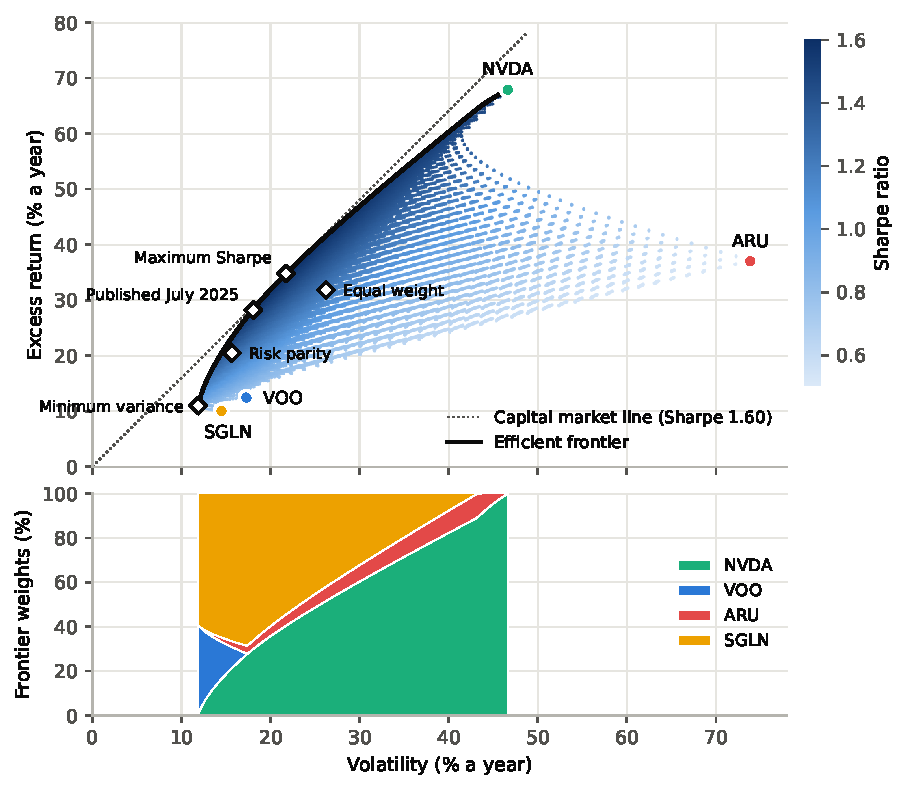
\includegraphics[width=0.74\linewidth]{figures/fig1_frontier.pdf}
\caption{The efficient frontier and the weights along it. Each dot is one of \gridN\ portfolios.}
\end{figure}

The corrections lower the optimum's Sharpe ratio from 1.87 to \msSharpe\ and move it from 29\% to \msNvda\% Nvidia, but its character is unchanged: Nvidia and gold, a little ARU, and no VOO (Table~3, Figure~1). The frontier holds VOO only at its low-risk end. Two features of the picture matter more than the optimum itself.

First, the optimum is flat. \gridShareTen\% of all portfolios have a Sharpe ratio within 10\% of the best, and among those within 5\% the Nvidia weight ranges from \nearNvdaLo\% to \nearNvdaHi\% and the gold weight from \nearSglnLo\% to \nearSglnHi\% (left panel of Figure~2). The data cannot distinguish sharply between portfolios that an investor would regard as very different.

Second, the published portfolio from the first version, although built from flawed inputs, sits almost on the corrected frontier with a Sharpe ratio of \vOneSharpe. The measurement errors changed the numbers more than the conclusion. What undermines the conclusion is in Sections~5 and~6.

\begin{figure}[ht]
\centering
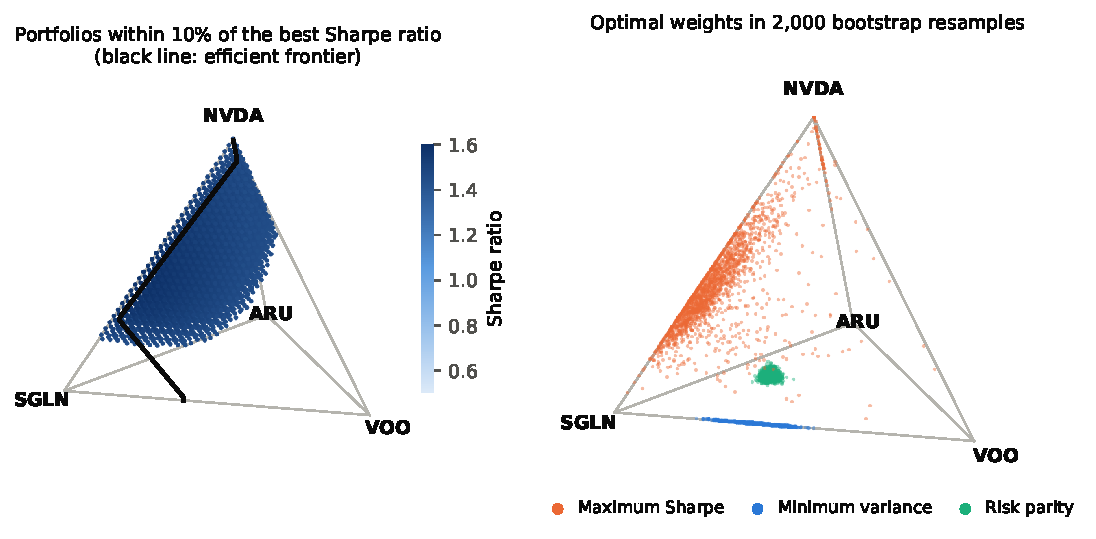
\includegraphics[width=0.92\linewidth]{figures/fig2_simplex.pdf}
\caption{The weight tetrahedron. Left: the portfolios within 10\% of the best in-sample Sharpe ratio. Right: the optimal portfolio under each rule in 2{,}000 bootstrap resamples of the estimation sample (Section~6).}
\end{figure}

\section{Tail risk}

Variance treats gains and losses alike. To see what that hides I compute each portfolio's expected shortfall (CVaR), the average loss in the worst 5\% of weeks, and divide it by the expected shortfall of a normal distribution with the same mean and volatility. A ratio above one means the left tail is fatter than variance suggests.

\begin{figure}[ht]
\centering
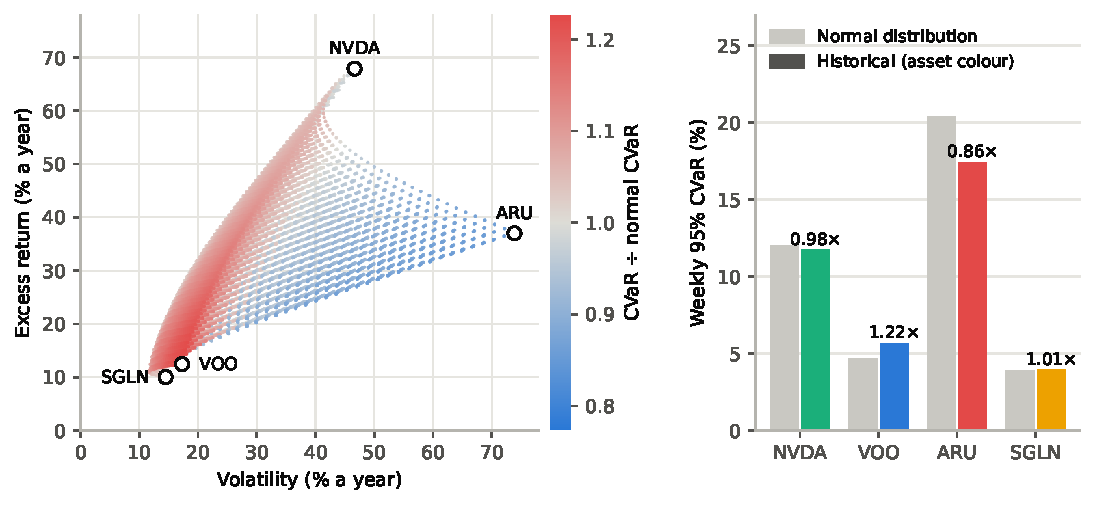
\includegraphics[width=0.92\linewidth]{figures/fig3_tail.pdf}
\caption{Left: historical CVaR relative to the normal benchmark for every portfolio. Right: the same comparison for the four assets.}
\end{figure}

The ratio is \ratioVoo\ for VOO and \ratioAru\ for ARU (Figure~3). The asset that looks safest by volatility has the worst tail relative to it, and the most volatile asset has a left tail that is thinner than a normal distribution's. The reason is skewness: $\skewVoo$ for VOO, whose large moves are crashes, and \skewAru\ for ARU, whose large moves are jumps upwards. This matches what I found on daily data in a separate study of ARU \citep{tok}, where the heavy tail is on the upside and a Gaussian model understates the risk of a short position, not a long one. Across the whole tetrahedron the ratio runs from \ratioMin\ to \ratioMax, and \ratioShareAbove\% of portfolios have a fatter left tail than the normal benchmark.

Does it change the answer? Not much. Minimising CVaR for each level of expected return \citep{rockafellar} gives a frontier whose CVaR is on average \cvarGain\% lower than the mean--variance frontier's, at the cost of \cvarVolCost\% more volatility, and the two sets of weights never differ by more than \cvarMaxGap\ percentage points. With 26 observations in the 5\% tail I would not read more into the differences than that.

\section{Out of sample}

\textbf{Rolling test.} Every four weeks from July 2018, I estimate means and covariances on the previous 156 weeks only, form four portfolios, and hold them for four weeks. This gives \rollWeeks\ weekly returns from \rollRebal\ rebalances in which no decision used later data.

\begin{table}[ht]
\centering\small
\caption{Rolling out-of-sample test, 27 July 2018 to 13 November 2026}
\begin{tabular}{lrrrrrr}
\toprule
 & Compound & Volatility & Sharpe & 90\% interval & Max.\ & Turnover \\
 & growth & & ratio & for Sharpe & drawdown & a year \\
\midrule
Maximum Sharpe & 27.0 & 28.8 & 0.88 & [0.30, 1.50] & -47 & 93 \\
Equal weight & 27.7 & 28.0 & 0.92 & [0.36, 1.47] & -33 & 49 \\
Risk parity & 22.6 & 17.5 & 1.10 & [0.54, 1.67] & -26 & 33 \\
Minimum variance & 14.9 & 13.1 & 0.92 & [0.40, 1.47] & -18 & 20 \\
\midrule
NVDA & 47.9 & 46.8 & 1.01 & & -66 & \\
VOO & 14.4 & 18.1 & 0.68 & & -32 & \\
ARU & 5.1 & 75.2 & 0.39 & & -84 & \\
SGLN & 14.6 & 16.2 & 0.75 & & -26 & \\
\bottomrule
\end{tabular}

\tabnote{Per cent except the Sharpe ratio. Intervals are from a stationary bootstrap of the weekly out-of-sample returns. Turnover is the share of the portfolio traded per year (one way). Transaction costs are not deducted.}
\end{table}

At each rebalance the maximum-Sharpe rule expected, on its own estimation window, a Sharpe ratio of \rollExpected\ on average. It realised \rollMs\ (Table~4). Equal weighting, which estimates nothing, realised \rollEw, and risk parity, which uses only the covariance matrix, \rollRp. The maximum-Sharpe portfolio also had the deepest drawdown (\rollMsDd\% against \rollRpDd\% for risk parity) and traded \rollMsTurn\% of its value a year against \rollRpTurn\%. This is the pattern documented by \citet{demiguel}, who find that optimised portfolios rarely beat equal weighting out of sample.

The ranking among the four rules is not statistically reliable. Eight years is a short sample for comparing Sharpe ratios: the 90\% interval for the maximum-Sharpe rule alone is [\rollMsLo, \rollMsHi], and for the difference between risk parity and maximum Sharpe it is [$\diffLo$, \diffHi] around an estimate of \diffEst. What the test does establish is narrower and, I think, sufficient: optimising on estimated means bought more turnover and more drawdown and no measurable gain.

\textbf{Hold-out.} The first version's portfolio was published in July 2025, so the period since is a test that could not have been tuned.

\begin{table}[ht]
\centering\small
\caption{Hold-out: portfolios fixed in July 2025, followed for \hoWeeks\ weeks}
\begin{tabular}{lrrrrr}
\toprule
 & Sharpe ratio & \multicolumn{4}{c}{1 August 2025 to 13 November 2026} \\
\cmidrule(lr){3-6}
 & to July 2025 & Total return & Volatility & Sharpe ratio & Max.\ drawdown \\
\midrule
Published July 2025 & 1.56 & 12.6 & 21.1 & 0.36 & -22 \\
Maximum Sharpe & 1.60 & 10.0 & 21.3 & 0.27 & -22 \\
Equal weight & 1.21 & 15.9 & 27.4 & 0.41 & -26 \\
Risk parity & 1.31 & 18.3 & 18.5 & 0.58 & -17 \\
Minimum variance & 0.93 & 19.1 & 15.4 & 0.70 & -12 \\
\midrule
NVDA & 1.46 & -5.9 & 33.7 & -0.08 & -30 \\
VOO & 0.72 & 20.1 & 12.0 & 0.92 & -8 \\
ARU & 0.50 & -20.7 & 78.6 & 0.11 & -63 \\
SGLN & 0.69 & 16.4 & 22.4 & 0.46 & -26 \\
\bottomrule
\end{tabular}

\tabnote{Portfolios are rebalanced to their July 2025 weights every four weeks. Returns, volatility and drawdown in per cent.}
\end{table}

\begin{figure}[ht]
\centering
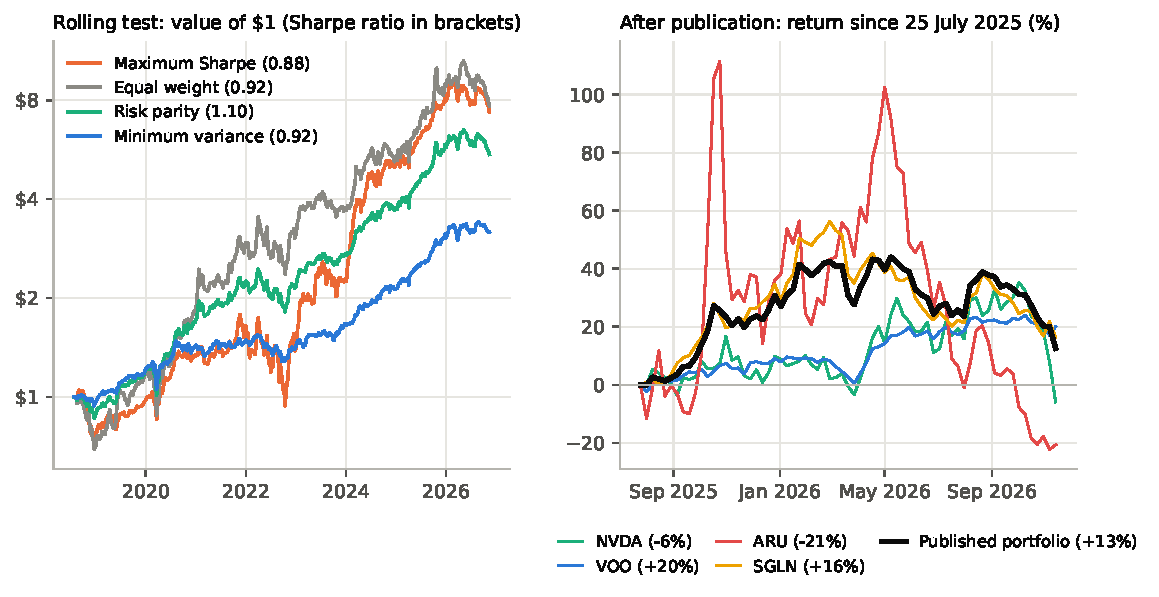
\includegraphics[width=0.95\linewidth]{figures/fig4_out_of_sample.pdf}
\caption{Left: the rolling test. Right: the four assets and the published portfolio since 25 July 2025.}
\end{figure}

The published portfolio returned \hoVOneRet\% with a Sharpe ratio of \hoVOneSharpe, against the \vOneSharpe\ it showed in sample, and fell \hoVOneDd\% from its peak (Table~5). VOO, to which it gave no weight, returned \hoVooRet\% with a Sharpe ratio of \hoVooSharpe\ and a drawdown of \hoVooDd\%. Nvidia lost \hoNvdaRet\% and ARU \hoAruRet\%.

I do not want to over-read this either. The verdict depends on the end date: at \hoEndAhead\ of the \hoEndTotal\ possible end dates from January 2026 onwards the published portfolio was ahead of VOO on total return, and at its peak in May 2026 it was up \hoPeak\%. It fell behind only in the last two weeks, when Nvidia fell by a fifth. What does not depend on the end date is that the portfolio's risk was misjudged. Gold, the ``defensive'' half of the barbell, had a volatility of \hoSglnVol\% in the hold-out against \isSglnVol\% before, and its correlation with ARU rose from \isCorrAruSgln\ to \hoCorrAruSgln. Covariances estimated over ten years were a poor description of the next sixteen months.

\section{Estimation error}

To see how much of the optimum is noise, I resample the \nWeeks\ weeks 2{,}000 times with a stationary block bootstrap \citep{politis}, which keeps volatility clustering intact, and recompute each portfolio on every resample (Table~6 and the right panel of Figure~2).

\begin{table}[ht]
\centering\small
\caption{Optimal weights and their 90\% bootstrap intervals (per cent)}
\begin{tabular}{lrrrr}
\toprule
 & NVDA & VOO & ARU & SGLN \\
\midrule
Maximum Sharpe & 40 & 0 & 5 & 54 \\
\quad 90\% interval & [21, 71] & [0, 15] & [0, 16] & [17, 73] \\
Minimum variance & 0 & 40 & 0 & 60 \\
\quad 90\% interval & [0, 0] & [32, 48] & [0, 0] & [52, 68] \\
Risk parity & 13 & 30 & 9 & 48 \\
\quad 90\% interval & [11, 14] & [28, 33] & [8, 10] & [46, 51] \\
\bottomrule
\end{tabular}

\end{table}

The maximum-Sharpe weight on Nvidia has a 90\% interval of \bootNvdaLo\% to \bootNvdaHi\%, and on gold of \bootSglnLo\% to \bootSglnHi\%. Gold is the largest holding in \bootSglnLargest\% of resamples and Nvidia in \bootNvdaLargest\%. The weights of the maximum-Sharpe portfolio are \bootRatio\ times as dispersed as those of the minimum-variance portfolio, and risk-parity weights barely move. This is the familiar result that expected returns are estimated far less precisely than covariances \citep{merton}, made visible: in the tetrahedron the maximum-Sharpe resamples smear along the whole Nvidia--gold edge while the other two rules stay in tight clusters. The Sharpe ratio of the optimum itself has an interval of \bootSharpeLo\ to \bootSharpeHi.

One result is stable. VOO receives less than 1\% in \bootVooZero\% of resamples. Within this decade, excluding the S\&P~500 was not an accident of the particular weeks drawn. But the bootstrap can only reshuffle the decade it is given, a decade in which one of the four assets compounded at \nvdaCagr\% a year. It measures sampling noise, not the chance that the next decade is different, and the hold-out is a reminder that it can be.

The same caution applies to single assets. VOO's Sharpe ratio is \srVoo\ and gold's \srSgln, and VOO's is the higher of the two in \bootVooSglnShare\% of resamples: ten years of data cannot rank them.

\section{Limitations}

\begin{itemize}
\item \textbf{The assets were chosen with hindsight.} I picked Nvidia in 2025 knowing how it had done. No test inside these four assets can remove that, and it is the largest reason not to treat any Sharpe ratio here as a forecast.
\item \textbf{Closing times still differ.} Weekly returns overlap by about 90\%, not fully; ARU's Friday close is still fifteen hours older than Nvidia's.
\item \textbf{No trading costs.} ARU trades on a coarse price grid on which one tick is about 2\% of the price \citep{tok}, so the turnover of the maximum-Sharpe rule would cost more than a flat assumption suggests. Including costs would widen its gap to the simpler rules.
\item \textbf{The tail estimates are thin.} A 5\% tail of \nWeeks\ weeks is 26 observations.
\item \textbf{Long only, four assets, one decade.}
\end{itemize}

\section{Conclusion}

The first version concluded that a concentrated barbell beats diversification. The corrected analysis reproduces that portfolio in sample and then fails to find the advantage where it could not have been fitted: not in the rolling test, and not in the sixteen months after publication. The bootstrap shows how loosely ten years of data pin the weights down. The conclusion I would draw now is the opposite of the one I drew then. With four assets and ten years of data, the part of the optimiser's answer that comes from expected returns is mostly noise, and the rules that ignore expected returns did at least as well with less risk and less trading.

The three-dimensional figures are more useful for this than for their original purpose. The tetrahedron shows the flat region of near-optimal portfolios and the scatter of resampled optima directly, and these are the two things a two-dimensional frontier hides.

\vspace{0.5\baselineskip}
{\small\noindent\textbf{Use of AI tools.} AI tools assisted in developing both versions of this project, including the code and, in this revision, the drafting of text. I take full responsibility for the content, and all errors are my own.\par}

\begin{thebibliography}{9}
\setlength{\itemsep}{2pt}\small
\bibitem[DeMiguel et~al.(2009)]{demiguel} DeMiguel, V., Garlappi, L. and Uppal, R. (2009). Optimal versus naive diversification: How inefficient is the $1/N$ portfolio strategy? \textit{Review of Financial Studies}, 22(5), 1915--1953.
\bibitem[Maillard et~al.(2010)]{maillard} Maillard, S., Roncalli, T. and Te\"iletche, J. (2010). The properties of equally weighted risk contribution portfolios. \textit{Journal of Portfolio Management}, 36(4), 60--70.
\bibitem[Markowitz(1952)]{markowitz} Markowitz, H. (1952). Portfolio selection. \textit{Journal of Finance}, 7(1), 77--91.
\bibitem[Merton(1980)]{merton} Merton, R.~C. (1980). On estimating the expected return on the market: An exploratory investigation. \textit{Journal of Financial Economics}, 8(4), 323--361.
\bibitem[Michaud(1989)]{michaud} Michaud, R.~O. (1989). The Markowitz optimization enigma: Is `optimized' optimal? \textit{Financial Analysts Journal}, 45(1), 31--42.
\bibitem[Politis and Romano(1994)]{politis} Politis, D.~N. and Romano, J.~P. (1994). The stationary bootstrap. \textit{Journal of the American Statistical Association}, 89(428), 1303--1313.
\bibitem[Rockafellar and Uryasev(2000)]{rockafellar} Rockafellar, R.~T. and Uryasev, S. (2000). Optimization of conditional value-at-risk. \textit{Journal of Risk}, 2(3), 21--41.
\bibitem[Tok(2026)]{tok} Tok, M. (2026). An empirical study in junior mining stock risk management: Weak-form efficiency tests and Value-at-Risk estimation with GARCH models. Working paper. \url{https://github.com/2008MT/aru-garch-var}
\end{thebibliography}

\end{document}
